\documentclass[10pt,a4paper,titlepage]{article}
\usepackage{latexsym}
\usepackage[a4paper,top=2.5cm,bottom=2.5cm,left=2.5cm,right=2.5cm]{geometry}
\usepackage[utf8x]{inputenc}
\usepackage{booktabs,caption,amsfonts,amssymb,fancyhdr, amsmath}
\usepackage[english]{babel}
\usepackage{indentfirst}
\usepackage{float}
\renewcommand*{\familydefault}{\sfdefault}
\usepackage{graphicx}
\usepackage{hyperref}
\usepackage{color}
\usepackage{subcaption}
\usepackage{listings}

\lstset{language=c++}
\lstset{backgroundcolor=\color{white}}
\lstset{frame=single}
\lstset{stringstyle=\ttfamily}
\lstset{keywordstyle=\color{red}\bfseries}
\lstset{commentstyle=\itshape\color{blue}}

\captionsetup[table]{position=top}
\pagestyle{headings}
\begin{document}
\begin{center}
{\LARGE \bfseries Computational Physics\par}
\vspace{0.5cm}
{\LARGE \bfseries Project 2 \par}
\end{center}

\vspace{1cm}

Academic year 2015-2016	 \hfill Giovanni Pederiva     

\begin{center}
\hrule height 2 pt
\end{center} 


\subsection*{Abstract}
The goal of this project was to solve Schr\"odinger's equation to find the wave function of a system composed by an electron in a harmonic oscillator 
well. The task could be written as an eigenvalue problem, so the implementation needed to solve the equation turned out to be the Jacobi method 
(or also known as Given's rotations) to diagonalize a matrix containing the discretization of the equation at different integration points. Once the 
matrix was written in a diagonal form I simply had to look at the lowest eigenstates and the relative eigenvectors, which gave the energy of the particle 
and the wave function respectively. There also is a closed form equation for the lowest eigenvalues to test the results with.\\
The second part of the project consisted in a similar problem, except that two interacting electron were to be considered inside the harmonic oscillator
potential. By rewriting Schr\"odinger's equation in terms of the center of mass it turned out that very few changes to the previous problem were needed, 
namely the potential function.\\
On the programming side, the goal of the project was to implement and test diagonalization algorithms and to develop some reproducible tests and 
benchmarks for our algorithm, to show that it is working properly.

\subsection*{Analysis Of The Problem}
The system we are considering is a 3-dimensional harmonic oscillator potential with spherical symmetry that acts on the electrons. The two particles 
interact with Coulomb's force. We will assume no angular components for the particles, only radial movement.\\
\paragraph*{One Particle System}
Let's first consider the system with only one particle, the radial Schr\"odinger's equation is then:
\begin{equation}
	-\frac{\hbar^2}{2 m} \left ( \frac{1}{r^2} \frac{d}{dr} r^2
  \frac{d}{dr} \right )\varphi(r) 
     + V(r) \varphi(r) = E \varphi(r).
\end{equation}
In this equation $\varphi (r)$ is the time independent wave function (note that since we are in spherical coordinates $r\in [0,\infty)$), 
the term $ \left (  \frac{1}{r^2} \frac{d}{dr} r^2 \frac{d}{dr} \right )\varphi(r) $ is the spatial second order derivative written in 
spherical coordinates, $V(r)$ is our potential, in this case it's the harmonic oscillator potential, so  $V(r) = \frac{1}{2}kr^2$ with $k=m\omega^2$ and 
$E$ is the energy of the harmonic oscillator in three dimensions. We have a closed form for the energy $E(r)$ that are eigenstates of the above wave 
function.
\[
E_{n}=  \hbar \omega \left(2n+\frac{3}{2}\right),
\]
\noindent with $n=0,1,2,\dots$. To simplify equation 1 and to make the discretization easier we put $u(r) = r~\varphi (r)$, this will also give bondary 
conditions that are easier to handle $u(0)=0$ and $u(\infty)=0$. So now the equation reads:
\begin{equation}
  -\frac{\hbar^2}{2 m} \frac{d^2}{dr^2}~u(r) + V(r)~u(r)  = E~u(r) .
\end{equation}
With the aim of getting to a dimensionless form for Schr\"odinger's equation we now introduce a dimensionless variable $\rho = (1/\alpha) r$ where 
$\alpha$ is a constant with dimension length and get:
\begin{equation}
  -\frac{\hbar^2}{2 m \alpha^2} \frac{d^2}{d\rho^2}~u(\rho) 
       + \frac{k}{2} \alpha^2\rho^2 ~ u(\rho)  = E~u(\rho) .
\end{equation}
We then multiply with $2m\alpha^2/\hbar^2$ on both sides and obtain
\begin{equation}
  -\frac{d^2}{d\rho^2} u(\rho) 
       + \frac{mk}{\hbar^2} \alpha^4\rho^2u(\rho)  = \frac{2m\alpha^2}{\hbar^2}E u(\rho) .
\end{equation}
The last step is to fix the constant $\alpha$ with a value that makes the potential coefficient equal to 1. So the choice is:
\[
\alpha = \left(\frac{\hbar^2}{mk}\right)^{1/4}.
\]
This simplification to a dimensionless equation however changed the energy eigenvalues of our original wave function. If we define 
\[
\lambda = \frac{2m\alpha^2}{\hbar^2}E,
\]
we can rewrite Schr\"odinger's equation as
\begin{equation}
  -\frac{d^2}{d\rho^2} u(\rho) + \rho^2u(\rho)  = \lambda u(\rho) .
\end{equation}
This is the first equation to solve numerically. In three dimensions we still have a closed form for the eigenvalues:
$\lambda_n = 3 + 4n$.


\paragraph*{Two Particle System}
We will now study the system made up with two electrons in a harmonic oscillator well interacting with each other via a repulsive Coulomb interaction.
If we consider no repulsive Coulomb interaction, we have the following Schr\"odinger equation in spherical coordinates, after having done some 
simplification as for the one particle system like setting $\psi(r_1, r_2) = r~\varphi (r_1, r_2)$.
\begin{equation}
\left(  -\frac{\hbar^2}{2 m} \frac{d^2}{dr_1^2} -\frac{\hbar^2}{2 m} \frac{d^2}{dr_2^2}+ \frac{1}{2}k r_1^2+ \frac{1}{2}k r_2^2\right)\psi(r_1,r_2) 
	 = E \psi(r_1,r_2) 
\end{equation}
\noindent Note that we deal with a two-electron wave function $\psi(r_1,r_2)$ and two-electron energy $E$. This equation can be separated in two, by 
considering the relative coordinate $r = r_1 - r_2$ and the center-of-mass coordinate $ R = 1/2(r_1+r_2)$.
The radial Schr\"odinger equation with the new coordinates now is:
\begin{equation}
\left(  -\frac{\hbar^2}{m} \frac{d^2}{dr^2} -\frac{\hbar^2}{4 m} \frac{d^2}{dR^2}+ \frac{1}{4} k r^2+  kR^2\right)\psi(r,R)  = E^{(2)} \psi(r,R).
\end{equation}
We now make the ansatz for the wave function $\psi(r,R) = u(r)\phi(R)$ so we end up having two separated wave functions, the which energies sum up in 
the end. If we now add a Coulomb potential of the form $V(r_1,r_2) = \frac{\beta e^2}{|r_1-r_2|}=\frac{\beta e^2}{r}$  only the relative 
equation will be changed, the center of mass will remain unchanged. 
The $r$-dependent Schr\"odinger equation becomes
\begin{equation}
\left(  -\frac{\hbar^2}{m} \frac{d^2}{dr^2}+ \frac{1}{4}k r^2+\frac{\beta e^2}{r}\right)u(r)  = E_r u(r).
\end{equation}
We can immediately see that this equation is very similar to the one we had for the one particle system, so we proceed in simplifying the equation as 
before by introducing dimensionless variable $\rho = r/\alpha$.  
\begin{equation}
  -\frac{d^2}{d\rho^2} u(\rho) 
       + \frac{1}{4}\frac{mk}{\hbar^2} \alpha^4\rho^2u(\rho)+\frac{m\alpha \beta e^2}{\rho\hbar^2}u(\rho)  = 
\frac{m\alpha^2}{\hbar^2}E_r u(\rho) .
\end{equation}
We now define 
\[
\omega^2=\frac{1}{4}\frac{mk}{\hbar^2} \alpha^4  ~~~~~~~~~~~~~~~~~~~~~ \alpha = \frac{\hbar^2}{m\beta e^2} ~~~~~~~~~~~~~~~~~~~~~
\lambda = \frac{m\alpha^2}{\hbar^2}E
\]
The parameter $\omega$ gives us an idea of the strength of the oscillator potential, $\lambda$ is the eigenvalue of the equation. We can now rewrite 
Schr\"odinger's equation in a very compact way:
\begin{equation}
  -\frac{d^2}{d\rho^2} u(\rho) + \left(\omega^2\rho^2 +\frac{1}{\rho} \right) u(\rho) = \lambda u(\rho).
\end{equation}

This analysis brought us to have two dimensionless differential equations. These represent two distinct systems and eigenvalue problems, however since 
their form is almost identical they can be solved with the same algorithm and the changes to the code required to compute the 2 paricle system are really
trivial.

\subsection*{Jacobi Method For Diagonalization}
All the next steps are applicable to both equation 5 or 10, the only change will be the term of the potential. This type of problems can be written very
easily in a matrix form. 
\[
{\bf Au } = \lambda {\bf u}
\]
Where ${\bf u }$ is the eigenvector representing the wave function corresponding to its eigenvalue energy level, and ${\bf A }$ is the matrix containing 
the discretized Schr\"odinger's equation. The first thing to do in order to compute the eigenvector of the equation is to discretize the second derivative
in the standard way:
\begin{equation}
    u''=\frac{u(\rho+h) -2u(\rho) +u(\rho-h)}{h^2} +O(h^2),
\end{equation} 
$h$ will be our step-length. Since the domain is definend from $0$ to $+\infty$ we need to set a maximum value for $\rho$. Since all the wave funnctions 
go to zero quite fast if we only want the first three eigenvalues a maximum value of $\rho_{max} = 7$ is enough. Since we require our matrix to be of a 
fixed size $n_{step}$ our step length  $h$ is fixed by $h=\frac{\rho_{max}}{n_{step}}$. 
We can now write the Schr\"odinger equation in a discretized form (for simplicity we put $u_i = u(ih)$):
\begin{equation}
-\frac{u_{i+1} -2u_i +u_{i-1} }{h^2}+V_iu_i  = \lambda u_i,
\end{equation}
where $V_i$ is the harmonic oscillator potential either alone or with the addition of the Coulomb potential term. If we write out the matrix we can also 
add in the potential terms. The matrix is now a tridiagonal matrix, and the equation can be written:
\[
    \left( \begin{array}{ccccccc} \frac{2}{h^2}+V_1 & -\frac{1}{h^2} & 0   & 0    & \dots  &0     & 0 \\
                                -\frac{1}{h^2} & \frac{2}{h^2}+V_2 & -\frac{1}{h^2} & 0    & \dots  &0     &0 \\
                                0   & -\frac{1}{h^2} & \frac{2}{h^2}+V_3 & -\frac{1}{h^2}  &0       &\dots & 0\\
                                \dots  & \dots & \dots & \dots  &\dots      &\dots & \dots\\
                                0   & \dots & \dots & \dots  &\dots       &\frac{2}{h^2}+V_{n_{\mathrm{step}}-2} & -\frac{1}{h^2}\\
                                0   & \dots & \dots & \dots  &\dots       &-\frac{1}{h^2} & \frac{2}{h^2}+V_{n_{\mathrm{step}}-1}

             \end{array} \right)  
                \left( \begin{array}{c} u_{1} \\
                                                              u_{2} \\
                                                              \dots\\ \dots\\ \dots\\
                                                              u_{n_{\mathrm{step}}-1}
             \end{array} \right)=\lambda \left( \begin{array}{c} u_{1} \\
                                                              u_{2} \\
                                                              \dots\\ \dots\\ \dots\\
                                                              u_{n_{\mathrm{step}}-1}
             \end{array} \right) 
\]
An eigen value problem is very easy to solve if the matrix we are considering is diagonal. The elements on the diagonal are the the eigenvalue itself. The
main idea is then to apply a sequence of rotations on the matrix in order to make it become diagonal. 
%These rotations are set in order to put to zero
%two elements of the matrix at a time, but might set a value that was previously zero to some other value. However the Frobenius norm is preserved since 
%the transformation is orthogonal and it is possible to show that at each itaration 
\begin{equation}
	{\bf (S^TAS)(S^T)x} = \lambda {\bf (S^T)x}
\end{equation}
The matrix ${\bf S}$ is of the form:
\[
\left( \begin{array}{ccccccccc} 1 & 0 & 0 & \dots & 0 & \dots & 0 & \dots & 0\\ 
								0 & 1 & 0 & \dots & 0 & \dots & 0 & \dots & 0\\ 
								0 & 0 & 1 & \dots & 0 & \dots & 0 & \dots & 0\\ 
								\dots & \dots & \dots & \dots & \dots & \dots & \dots & \dots & \dots\\ 
								0 & 0 & 0 & \dots & cos(\theta) & \dots & sin(\theta) & \dots & 0 \\ 
								\dots & \dots & \dots & \dots & \dots & \dots & \dots & \dots & \dots\\ 
								0 & 0 & 0 & \dots & -sin(\theta) & \dots & cos(\theta) & \dots & 0\\ 
								\dots & \dots & \dots & \dots & \dots & \dots & \dots & \dots & \dots\\ 
								0 & 0 & 0 & \dots & 0 & \dots & 0 & \dots & 1\\ 
                                

             \end{array} \right)  
\]
The transformation is chosen by first searching through the matrix to find the largest non diagonal elements, then the angle $\theta$ is computed to make 
those elements become 0. Then the triple matrix product is computed. Since the transformation matrix is very simple a simple multiplication scheme can 
be derived. If we call $b_{i,j}$ the elements of the transformed matrix and let $k, l$ be the indexes of the largest non diagonal element:
\begin{equation}
\begin{array}{cc}
b_{ii} = &a_{ii}~~~~for~i \neq k, i \neq l \hfill\\
b_{ik} = &a_{ik} cos\theta − a_{il} sin\theta\hfill\\  
b_{il} = &a_{il} cos\theta + a_{ik} sin\theta \hfill\\
b_{kk} = &a_{kk} cos^2 \theta − 2a_{kl} cos \theta sin \theta + a_{ll} sin^2 \theta\hfill\\
b_{ll} = &a_{ll} cos^2 \theta + 2a_{kl} cos \theta sin \theta + a_{kk} sin^2 \theta\hfill\\
b_{kl} = &(a_{kk} − a_{ll} )cos \theta sin \theta + a_{kl} (cos^2 \theta − sin^2 \theta )\hfill
\end{array} 
\end{equation}
The last equation is the one that has to be set to zero to find the angle $\theta$. It can be rewritten as $t^2 + 2\tau - 1 = 0$ where $t = tan\theta$ and
$\tau = \frac{a_ll - a_kk}{2a_{kl}}$. From the tangent we can easily get the cosine $cos\theta = \frac{1}{\sqrt{1+t^2}}$ and sine $sin\theta = tan\theta
cos\theta$. 
After every rotation we must rotate also the eigenvectors. From equation 13 we easily see how, if we start with an orthnormal basis of vectors, that could
be for example the identy matrix if we consider every column as a vector, by applying these rotations we get to the eigenvectors we are looking for. 
The explicit for of these rotations reads:
\begin{equation}
\begin{array}{cc}
u'_{ik} = &u_{ik} cos\theta − u_{il} sin\theta\hfill\\  
u'_{il} = &u_{il} cos\theta + u_{ik} sin\theta \hfill\\
\end{array} 
\end{equation}
To make the algorithm stop we must impose a threshold for the sum of all non diagonal matrix elements. We will set it to $10^{-8}$ which means that the
matrix is not really diagonal, but all the elements non on the diagonal are very close to zero.\\
We have now a very easy to implement algorithm that I'll summarize here:
\begin{itemize}
\item choose a mesh size for the matrix $n_{steps}$, the maximum point of intefration $\rho_{max}$ and compute $h$
\item create the starting $n\times n$ matrix containing the Scr\"odinger's equation and the identity matrix for the eigenvectors.
\item find the largest non-diagonal element of the matrix $a_{kl}$
\item compute the angle $\theta$ to set $a_{kl} = 0$
\item apply the rotation scheme to the matrix
\item apply the rotation scheme to the eigenvectors
\item calculate the sum of all non diagonal methods and check if it's smaller then the required tolerance.
 
\end{itemize}

\subsection*{Implementation Tests}
I wrote a $C++$ code to solve this problem\footnote{The full code can be found on GitHub \url{https://github.com/GioPede/FYS3150/blob/master/Project2
/main.cpp}} and developed a function that given a certain matrix it returned it's diagonalization. While developing the code some tests were engineered 
to make sure that the program was working properly. The first test consisted in giving as an argument for the function a diagonal matrix. The function 
should then exit without doing anything. \\
Another test was to set up a very simple  $2\times 2$ matrix. This should be diagonalized in just one iteration by definition. If these requirements 
were not met, then it meant that the program wasn't working properly, and exited before starting doing the real problem calculation.
As a further test we had the closed form for the eigenvalues of the one particle system to compare our results with, if some other values appeared, then
there was an error in our code.

\subsection*{Numerical Results}
After the algorithm had been implemented I ran some tests to find the three lowest energy wave functions on both systems. Here are the plots for the 
single electron system:\\
\begin{minipage}{0.5\textwidth}
	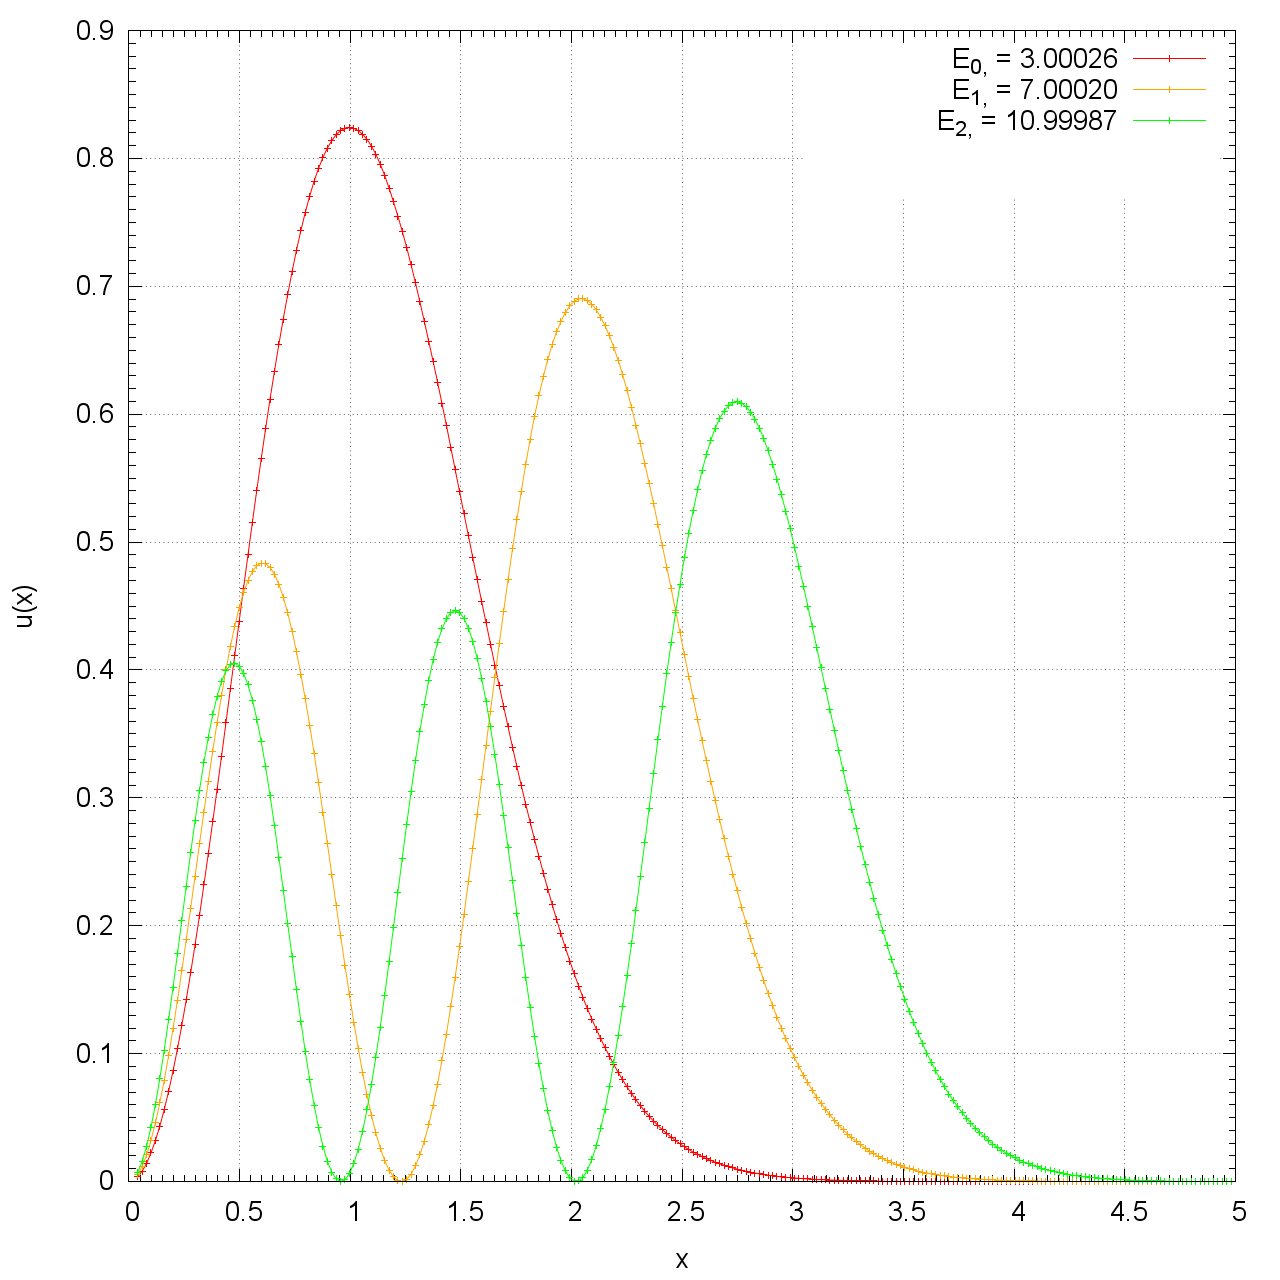
\includegraphics[width=0.8\columnwidth]{plot_harm_u.png}
    \captionof{figure}{{\footnotesize  One particle system. Plot of the function $|u(x)|^2$ \\for the first three eigenvalues.}}
\end{minipage}
\begin{minipage}{0.5\textwidth}
	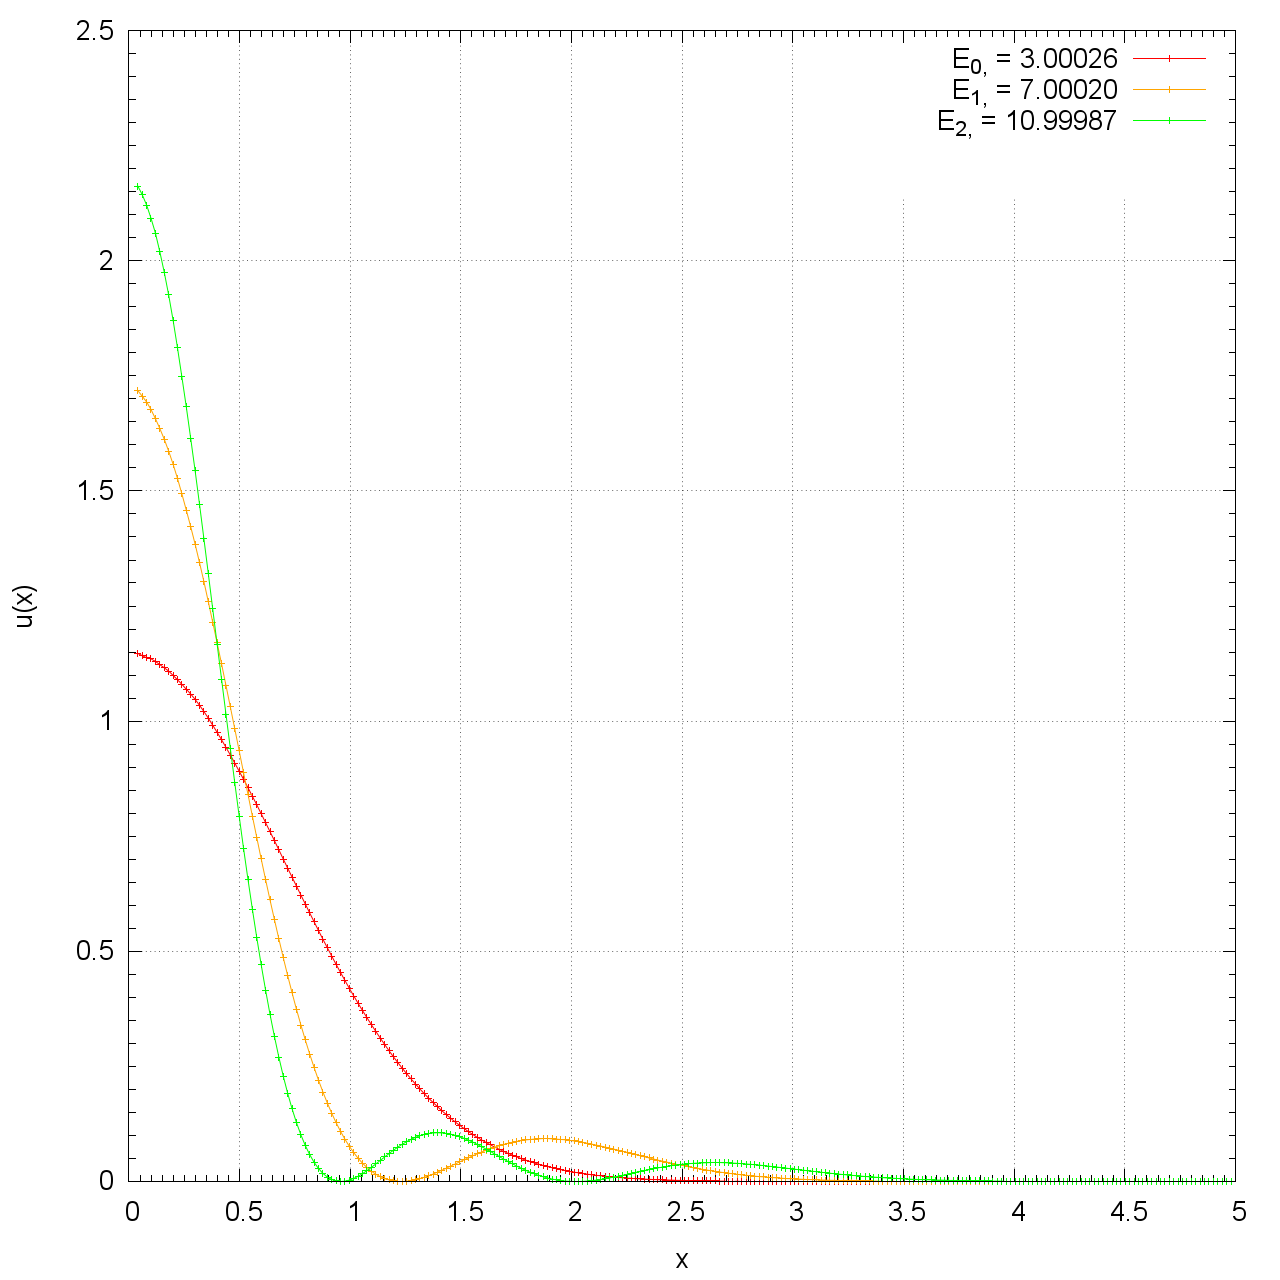
\includegraphics[width=0.8\textwidth]{plot_harm.png}
    \captionof{figure}{{\footnotesize  One particle system. Plot of the function \\$|\psi(x)|^2 = |u(x)| ^2 / \rho ^2$ for the first three eigenvalues}}
\end{minipage}\\
And the ones for the two particle system with $\omega = 0.1$ for the relative distance only:\\
\begin{minipage}{0.5\textwidth}
	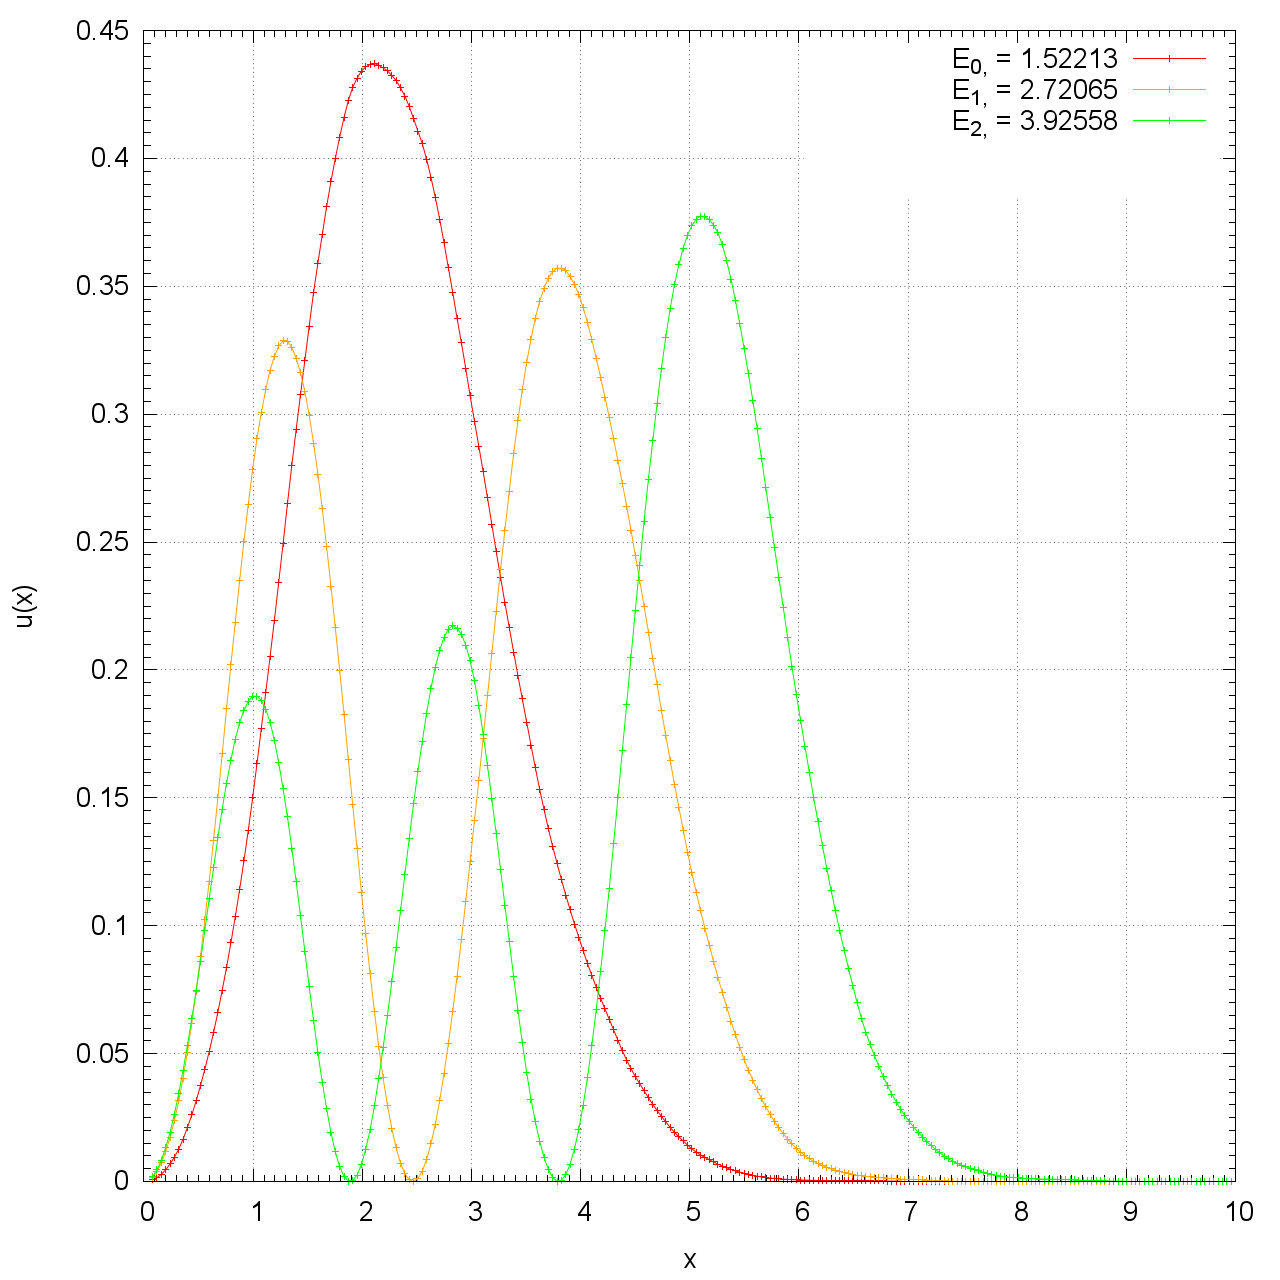
\includegraphics[width=0.8\columnwidth]{plot_2e_u.png}
    \captionof{figure}{{\footnotesize  Two particle system. Plot of the function $|u(x)|^2$ \\for the first three eigenvalues.}}
\end{minipage}
\begin{minipage}{0.5\textwidth}
	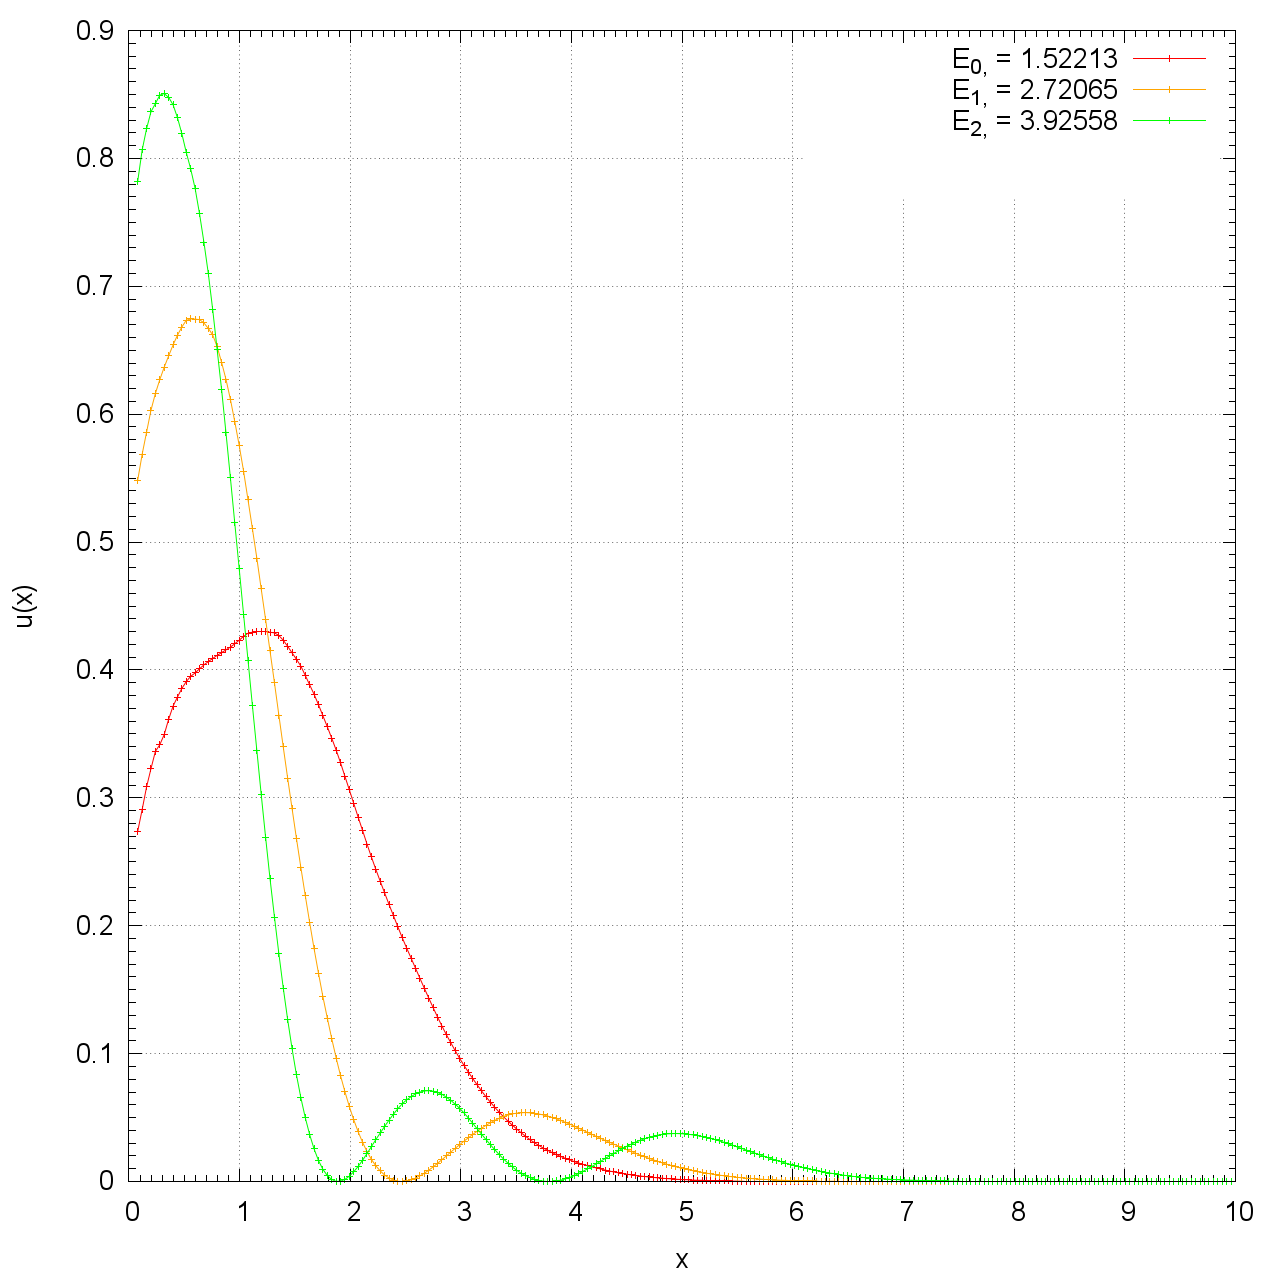
\includegraphics[width=0.8\textwidth]{plot_2e.png}
    \captionof{figure}{{\footnotesize  Two particle system. Plot of the function \\$|\psi(x)|^2 = |u(x)| ^2 / \rho ^2$ for the first three eigenvalues}}
\end{minipage}\\
The first two plots show also the values of the eigenvalues of which we had a closed form. They are equal to the ones that we were expecting with four
leading digits:\\
\begin{center}
\begin{tabular}{|c|c|c|}
\hline
       &  Expected &  Numerical\\\hline
$E_0$  &         3 &  3.00026  \\\hline
$E_1$  &         7 &  7.00020  \\\hline
$E_2$  &        11 & 10.99987  \\\hline
\end{tabular}
\captionof{figure}{{\footnotesize  Expected eigenvalues and numerically found ones.}}
\end{center}
To achive this precision however it was necessary to set up a matrix of dimension 250 in the interval $(0,5)$ and due to it's dimension it required 
approximately 40000 iterations, or in seconds $\simeq 5.5 s$. This shows how inefficient this method is, especially beacuse we had a very simple matrix
as a tridiagonal one, so a better and specific algorithm could have been used, like Francis' algorithm or the QL algorithm with implicit shifts found
on "Numerical Recipes" by William H. Press (function name \texttt{tqli}). I made an implementation of the latter and compared the number of total 
iterations along the matrix of the two methods. Here are the results:\\
\begin{center}
\begin{tabular}{|c|c|c|}
\hline
Matrix Dimension  &  Jacobi Method &  $~~~~$ \texttt{tqli}$~~~~$ \\\hline
100  &   7052  &  12474  \\\hline
150  &   16905 &  27893  \\\hline
200  &   31015 &  48997  \\\hline
250  &   49559 &  75149  \\\hline
\end{tabular}
\captionof{figure}{{\footnotesize  Total matrix iterations of the two methods related to the matrix dimension.}}
\end{center}
There is a clear difference between the two methods and the most of the difference is in the fact that the Jacobi method requires to look through the 
entire matrix at every step to look for the largest non-diagonal element, while the QL algorithm doesn't. This decreases the number of rotations needed
but since each iterations requires approximately $2n$ operations for both methods and a single matrix sweep to look for the largest elements reqires $n^2$
operations, the  \texttt{tqli} is still much faster. For the same dimensionality of 250 it took for example $5.62586$ seconds for the Jacobi method
and $0.44235$s for the QL algorithm; this algorithm took 5 seconds to diagonalize a matrix of size 1000, four times larger than the one other method could 
do in the same time. The Lanczos' method would be even faster at find the eigenvalues, but it does not give any easy to implement algorithm for 
eigenvectors.\\
As a last test I ran a series of simulation for the two particle system in which the parameter $\omega$ changed between the values 0.01, 0.5, 1 and 5.
Here's a plot of the different wave functions.  \\
\begin{minipage}{0.5\textwidth}
	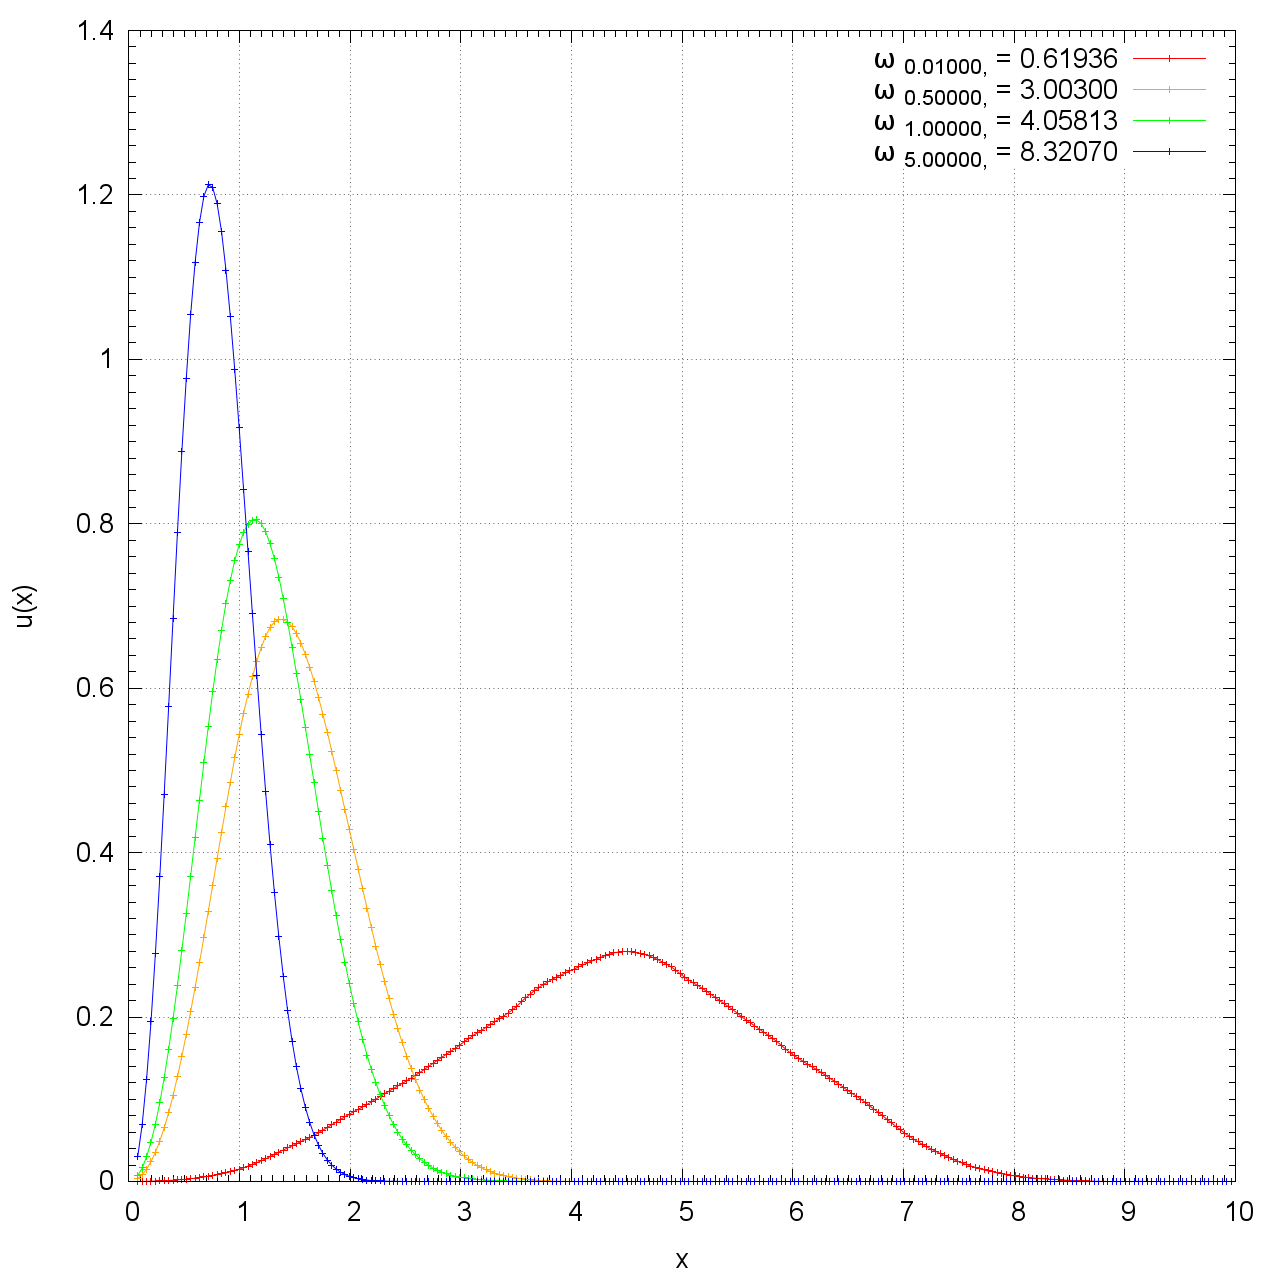
\includegraphics[width=0.8\columnwidth]{plot_omega_u.png}
    \captionof{figure}{{\footnotesize  $|u(x)|^2$ for the two particle system with different values of $\omega$}}
\end{minipage}
\begin{minipage}{0.5\textwidth}
	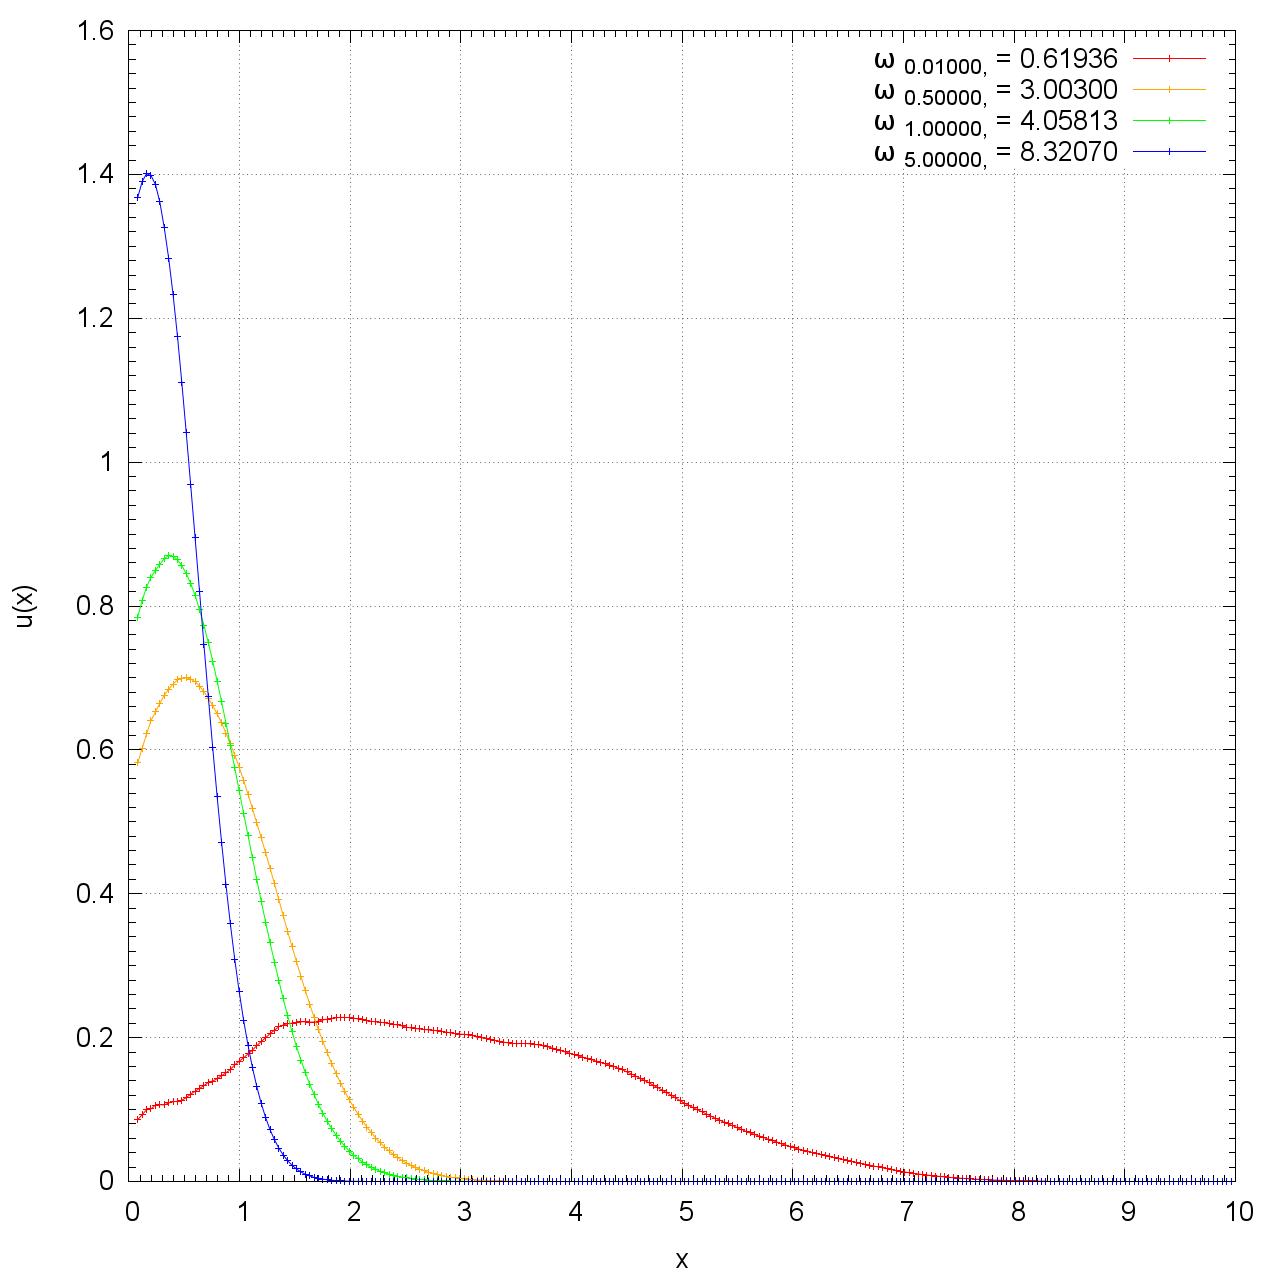
\includegraphics[width=0.8\textwidth]{plot_omega.png}
    \captionof{figure}{{\footnotesize  $|\psi(x)|^2$ for the two particle system with different values of $\omega$}}
\end{minipage}\\
As expected if the harmonic oscillator is very weak if compared to the Coulomb interaction then the particles tend to be further apart, but if it gets 
stronger then the wave function tends to the one of the one particle system. The strangeness in slope for the $|\psi(x)|^2$ for $\omega = 0.01$ can be
due to the roundoff errors and machine error.

\subsection*{Conclusions}
This project showed that some quantum mechanical systems can be solved numerically by using diagonalization algorithms. The easiest to implement is the 
Jacobi algorithm which is very stable but requires a lot of computation time. The algorithm \texttt{tqli} found in literature applies more similarity
transformation, but is much faster in computation time. \\
The application of these methods to Schr\"odinger equation in the case of a single electron in a three dimensional harmonic oscillator well
gave us the expected results, as it did for the two electron system when changing the value $\omega$. The behaviour of the probability
density function which has been found is the one we expected, also in comparison to its corresponding one without the Coulomb interaction. 
\end{document}